
\documentclass[11pt,a4paper,UTF8]{ctexart}

\usepackage[T1]{fontenc}
\usepackage[utf8]{inputenc}
\usepackage{authblk}

\usepackage{ctex} %导入中文包
\usepackage{tocvsec2}

\usepackage{tabularx}
\usepackage{booktabs} 
\usepackage{multirow}
\usepackage{bbding}
\usepackage{float}
\usepackage{xspace}
\usepackage[none]{hyphenat}

\usepackage{graphicx}
\usepackage{subfigure}

\usepackage{subfiles} %使用多文件方式进行

\usepackage{geometry} %设置页边距的包
\geometry{left=2.5cm,right=2cm,top=2.54cm,bottom=2.54cm} %设置书籍的页边距

\usepackage{url}
\usepackage{hyperref}  %制作pdf的目录
\hypersetup{hidelinks, %去红框
	colorlinks=true,
	allcolors=black,
	pdfstartview=Fit,
	breaklinks=true
}

% 调整itemlist中的行间距
\usepackage{enumitem}
\setenumerate[1]{itemsep=0pt,partopsep=0pt,parsep=\parskip,topsep=5pt}
\setitemize[1]{itemsep=0pt,partopsep=0pt,parsep=\parskip,topsep=5pt}
\setdescription{itemsep=0pt,partopsep=0pt,parsep=\parskip,topsep=5pt}

% 超链接样式设置
\usepackage{hyperref}
\hypersetup{
	colorlinks=true,
	linkcolor=blue,
	filecolor=blue,
	urlcolor=blue,
	citecolor=cyan,
}

\usepackage{indentfirst}

\usepackage{listings}
\usepackage[usenames,dvipsnames,svgnames, x11names]{xcolor}

\usepackage{tcolorbox}

%展示代码
\definecolor{mygreen}{rgb}{0,0.6,0}
\definecolor{mygray}{rgb}{0.5,0.5,0.5}
\definecolor{mymauve}{rgb}{0.58,0,0.82}
\lstset{
	backgroundcolor=\color{blue!3!white}, 
	%basicstyle = \footnotesize,  
	basicstyle=\tt,     
	breakatwhitespace = false,        
	breaklines = true,                 
	captionpos = b,                    
	commentstyle = \color{mygreen}\bfseries,
	extendedchars = false,             
	frame =shadowbox, 
	framerule=0.5pt,
	keepspaces=true,
	keywordstyle=\color{blue}\bfseries, % keyword style
	language = C++,                     % the language of code
	otherkeywords={string}, 
	numbers=left, 
	numbersep=5pt,
	numberstyle=\tiny\color{mygray},
	rulecolor=\color{black},         
	showspaces=false,  
	showstringspaces=false, 
	showtabs=false,    
	stepnumber=1,         
	stringstyle=\color{mymauve},        % string literal style
	tabsize=2,          
	title=\lstname                      
}

\usepackage{tikz}

\begin{document}
	%\maketitle
	
	\begin{center}
		%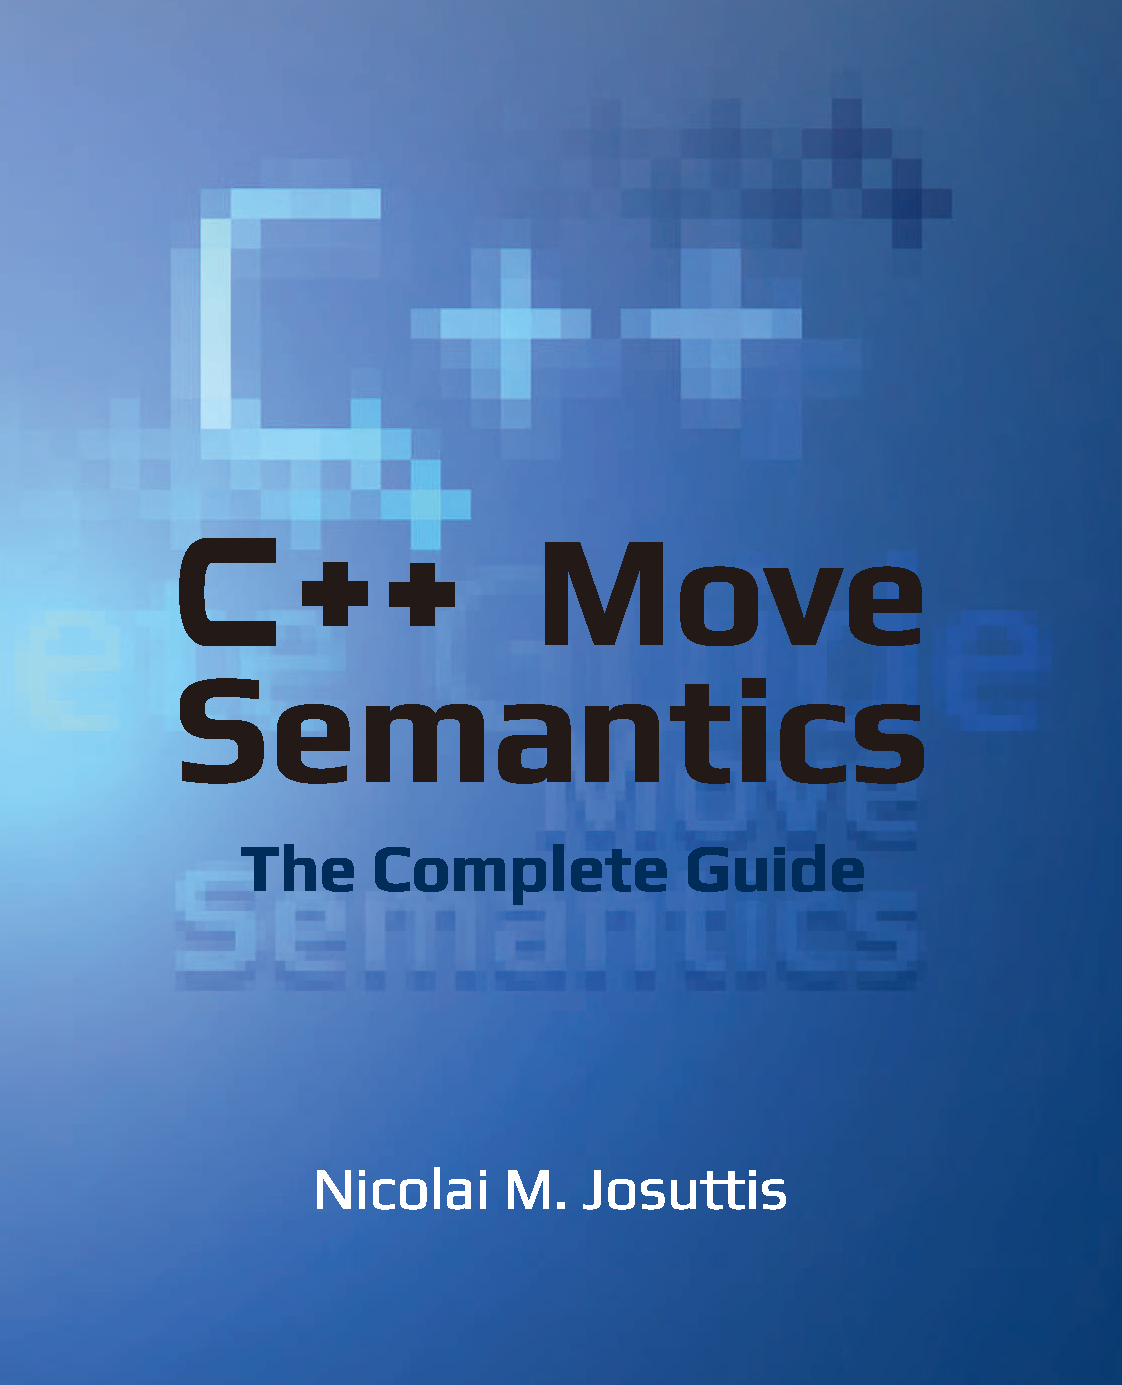
\includegraphics[width=\textwidth,height=\textheight,keepaspectratio]{cover.png}
		\begin{tikzpicture}[remember picture, overlay, inner sep=0pt]
			\node at (current page.center) 
			{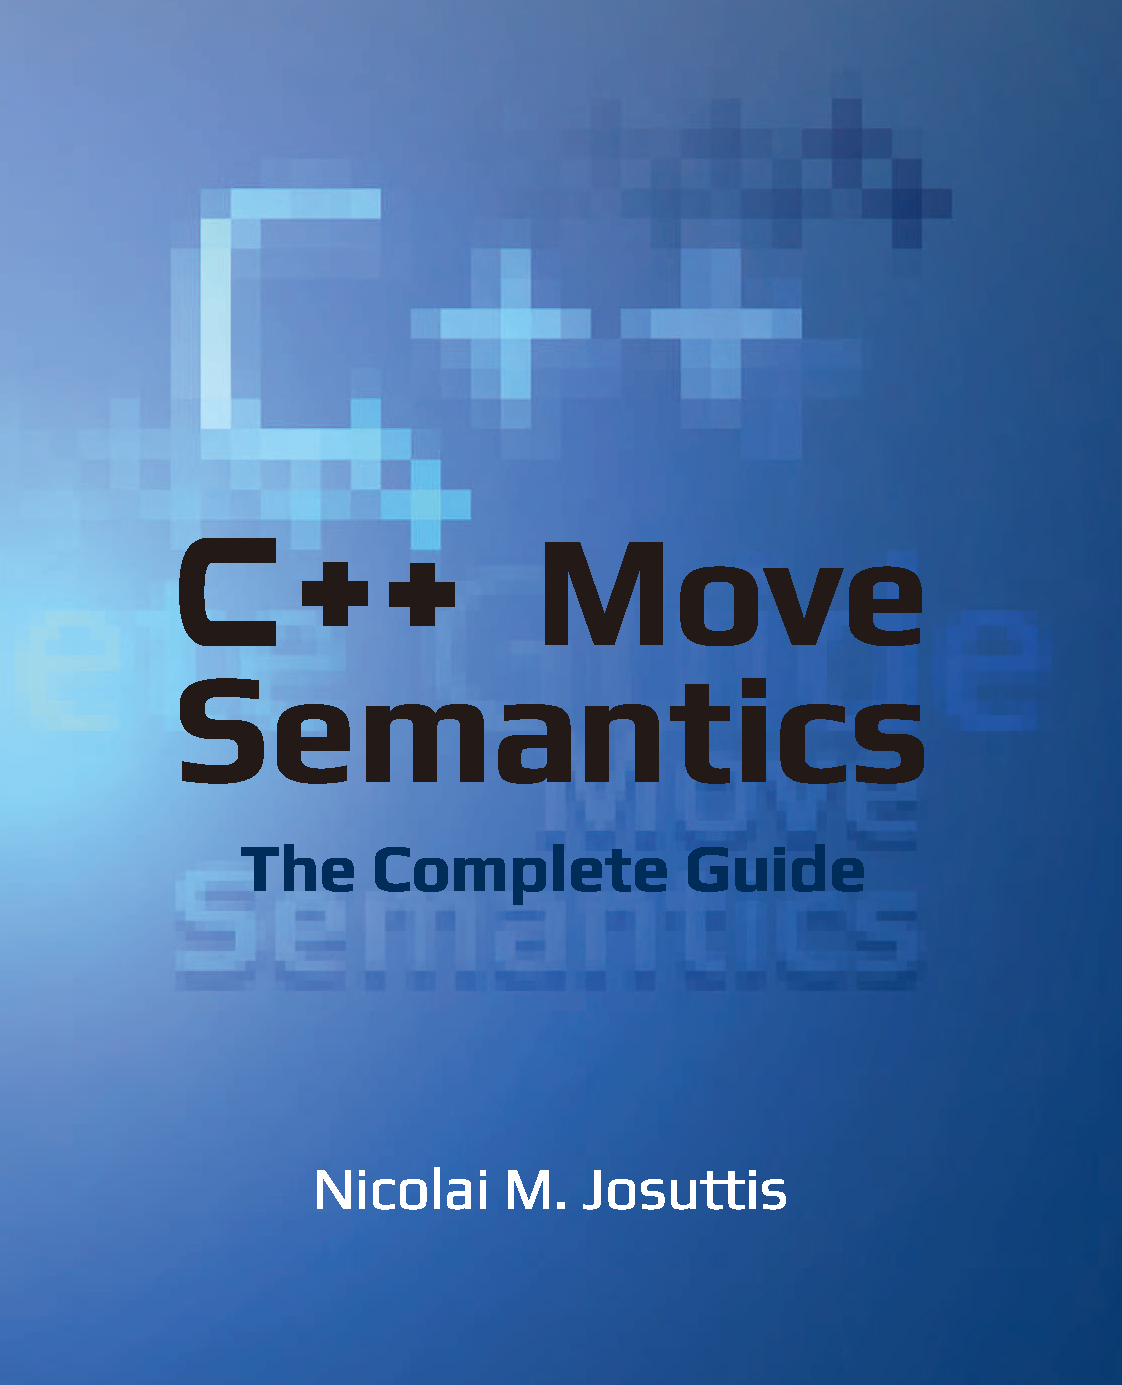
\includegraphics[width=\paperwidth, height=\paperheight, keepaspectratio=false]{cover.png}};
		\end{tikzpicture}
		\newpage
		\huge
		\textbf{Learn LLVM 12} 
		\\[9pt]
		\normalsize
		A beginner's guide to learning LLVM compiler tools and core libraries with C++ 
		\\[10pt]
		\normalsize 
		作者: Kai Nacke
		\\[8pt]
		\normalsize
		译者;陈晓伟
	\end{center}
	
	\hspace*{\fill} \\ %插入空行
	\noindent\textbf{本书概述}\ \par

	学习如何构建和使用编译器,包括前端、流水线优化和利用LLVM核心库的强大功能构建新的后端编译器。\par
	
	LLVM是为了弥合编译器理论和实际开发之间的差异而出现的。它提供了模块化的代码库和先进的工具,帮助开发人员轻松地构建编译器。本书提供了对LLVM的介绍,帮助读者在各种情况下构建和使用编译器。\par
	
	本书将从配置、构建和安装LLVM库、工具和外部项目开始。接着,向您介绍LLVM的设计,以及在每个编译器阶段(前端、优化器和后端)的实际工作方式。以实际编程语言为例,学习如何使用LLVM开发前端编译器,并生成LLVM IR,将其交给优化流水线,并从中生成机器码。后面的章节将展示如何扩展LLVM,以及LLVM中的指令选择是如何工作的。在了解如何为LLVM开发新的后端编译器之前,将重点讨论即时编译问题和LLVM提供的JIT编译的支持情况。\par
	
	阅读本书后,您将获得使用LLVM编译器开发框架的实际经验,并得到一些具有帮助性的实际示例和源代码片段。\par
	
	\textbf{关键特性}:\par
	
	\begin{itemize}
		\item 学习如何有效地使用LLVM
		\item 理解LLVM编译器的高级设计,并将原则应用到自己的编译器中
		\item 使用基于编译器的工具来提高C++项目的代码质量
	\end{itemize}
	
	\textbf{内容纲要}:\par
	
	\begin{itemize}
		\item 配置、编译和安装LLVM框架
		\item 理解LLVM源码的结构
		\item 了解在项目中可以使用LLVM做什么
		\item 探索编译器是如何构造的,并实现一个小型编译器
		\item 为通用源语言构造生成LLVM IR
		\item 建立优化流水线,并根据自己的需要进行调整
		\item 使用转换通道和Clang工具对LLVM进行扩展
		\item 添加新的机器指令和完整的后端编译器
	\end{itemize}
	
	
	\hspace*{\fill} \\ %插入空行
	\noindent\textbf{作者简介}\ \par
	
	\textbf{Kai Nacke}是一名专业IT架构师,目前居住在加拿大多伦多。毕业于德国多特蒙德技术大学的计算机科学专业。他关于通用哈希函数的毕业论文,被评为最佳论文。\par
	
	他在IT行业工作超过20年,在业务和企业应用程序的开发和架构方面有丰富的经验。他在研发一个基于LLVM/Clang的编译器。\par
	
	几年来,他一直是LDC(基于LLVM的D语言编译器)的维护者。在Packt出版过《D Web Development》一书,他也曾在自由和开源软件开发者欧洲会议(FOSDEM)的LLVM开发者室做过演讲。\par
	
	\hspace*{\fill} \\ %插入空行
	\noindent\textbf{审评者介绍}\ \par
	
	\textbf{Suyog Sarda}是一名专业的软件工程师和开源爱好者,专注于编译器开发和编译器工具,是LLVM开源社区的积极贡献者。他毕业于了印度浦那工程学院,具有计算机技术学士学位。Suyog还参与了ARM和X86架构的代码性能改进,一直是Tizen项目编译团队的一员,对编译器开发的兴趣在于代码优化和向量化。之前,他写过一本关于LLVM的书,名为《LLVM Cookbook》,由Packt出版。除了编译器,Suyog还对Linux内核开发感兴趣。他在迪拜Birla Institute of Technology的2012年IEEE Proceedings of the International Conference on Cloud Computing, Technologies, Applications, and Management上发表了一篇题为《VM pin and Page Coloring Secure Co-resident Virtualization in Multicore Systems》的技术论文。

	
	\hspace*{\fill} \\ %插入空行
	\noindent\textbf{本书相关}\ \par
	\begin{itemize}
		\item github翻译地址:\url{https://github.com/xiaoweiChen/Learn-LLVM-12}
		\item 本书代码:\url{https://github.com/PacktPublishing/Learn-LLVM-12}
	\end{itemize}
	\newpage
	
	
	\begin{center}
		\vspace*{\fill}
		写书是一项具有挑战性的任务。尤其是正计划移居加拿大时,突然一场流行病袭击了世界,改变了一切。\par
		
		\hspace*{\fill} \par
		
		Packt的团队在写作上给予指导,也对我缓慢的写作速度表示理解,并一直激励我坚持下去。我非常非常感谢他们。\par
		
		\hspace*{\fill} \par
		
		没有家人的支持,就不可能有这本书。谢谢对我的信心!\par
		
		\vspace*{\fill}
	\end{center}
	
	\newpage
	
	\pagestyle{empty}
	\subfile{content/Preface.tex}
	
	\tableofcontents
	\newpage
	
	\setsecnumdepth{section}
	
	\color{white}
	\section*{\zihao{1} 1 构建LLVM}
	\pagecolor{mygray}
	\addcontentsline{toc}{section}{1 构建LLVM}
	\subfile{content/1/Part-1.tex}
	\color{black}
	\pagecolor{white}
	
	\subsection*{\zihao{2} 第1章\hspace{0.5cm}安装LLVM}
	\addcontentsline{toc}{subsection}{第1章\hspace{0.5cm}安装LLVM}
	\subfile{content/1/chapter1/0.tex}
	
		\subsubsection*{\zihao{3} 相关准备}
		\addcontentsline{toc}{subsubsection}{相关准备}
		\subfile{content/1/chapter1/1.tex}
		
		\subsubsection*{\zihao{3} 使用CMake构建}
		\addcontentsline{toc}{subsubsection}{使用CMake构建}
		\subfile{content/1/chapter1/2.tex}
		
		\subsubsection*{\zihao{3} 定制化构建}
		\addcontentsline{toc}{subsubsection}{定制化构建}
		\subfile{content/1/chapter1/3.tex}
		
		\subsubsection*{\zihao{3} 总结}
		\addcontentsline{toc}{subsubsection}{总结}
		\subfile{content/1/chapter1/4.tex}
		
	\subsection*{\zihao{2} 第2章\hspace{0.5cm}浏览LLVM}
	\addcontentsline{toc}{subsection}{第2章\hspace{0.5cm}浏览LLVM}
	\subfile{content/1/chapter2/0.tex}
		\subsubsection*{\zihao{3} 相关代码}
		\addcontentsline{toc}{subsubsection}{相关代码}
		\subfile{content/1/chapter2/1.tex}
		\subsubsection*{\zihao{3} LLVM代码的内容}
		\addcontentsline{toc}{subsubsection}{LLVM代码的内容}
		\subfile{content/1/chapter2/2.tex}
		\subsubsection*{\zihao{3} LLVM的项目结构}
		\addcontentsline{toc}{subsubsection}{LLVM的项目结构}
		\subfile{content/1/chapter2/3.tex}
		\subsubsection*{\zihao{3} 使用LLVM创建自己的项目}
		\addcontentsline{toc}{subsubsection}{使用LLVM创建自己的项目}
		\subfile{content/1/chapter2/4.tex}
		\subsubsection*{\zihao{3} 针对不同的CPU架构}
		\addcontentsline{toc}{subsubsection}{针对不同的CPU架构}
		\subfile{content/1/chapter2/5.tex}
		\subsubsection*{\zihao{3} 总结}
		\addcontentsline{toc}{subsubsection}{总结}
		\subfile{content/1/chapter2/6.tex}
		
	\subsection*{\zihao{2} 第3章\hspace{0.5cm}编译器结构}
	\addcontentsline{toc}{subsection}{第3章\hspace{0.5cm}编译器结构}
	\subfile{content/1/chapter3/0.tex}
		\subsubsection*{\zihao{3} 相关代码}
		\addcontentsline{toc}{subsubsection}{相关代码}
		\subfile{content/1/chapter3/1.tex}
		\subsubsection*{\zihao{3} 编译器的构建块}
		\addcontentsline{toc}{subsubsection}{编译器的构建块}
		\subfile{content/1/chapter3/2.tex}
		\subsubsection*{\zihao{3} 算术表达式语言}
		\addcontentsline{toc}{subsubsection}{算术表达式语言}
		\subfile{content/1/chapter3/3.tex}
		\subsubsection*{\zihao{3} 语法分析}
		\addcontentsline{toc}{subsubsection}{语法分析}
		\subfile{content/1/chapter3/4.tex}
		\subsubsection*{\zihao{3} 语义分析}
		\addcontentsline{toc}{subsubsection}{语义分析}
		\subfile{content/1/chapter3/5.tex}
		\subsubsection*{\zihao{3} 使用LLVM后端编译器生成代码}
		\addcontentsline{toc}{subsubsection}{使用LLVM后端编译器生成代码}
		\subfile{content/1/chapter3/6.tex}
		\subsubsection*{\zihao{3} 总结}
		\addcontentsline{toc}{subsubsection}{总结}
		\subfile{content/1/chapter3/7.tex}
    
    \color{white}
	\section*{\zihao{1} 2 从源码到机器码}
	\pagecolor{mygray}
	\addcontentsline{toc}{section}{2 从源码到机器码}
	\subfile{content/2/Part-2.tex}
	\color{black}
	\pagecolor{white}
	
	\subsection*{\zihao{2}第4章\hspace{0.5cm}将源文件转换为抽象语法树}
	\addcontentsline{toc}{subsection}{第4章\hspace{0.5cm}将源文件转换为抽象语法树}
	\subfile{content/2/chapter4/0.tex}
		\subsubsection*{\zihao{3} 相关代码}
		\addcontentsline{toc}{subsubsection}{相关代码}
		\subfile{content/2/chapter4/1.tex}
		\subsubsection*{\zihao{3} 定义一种编程语言}
		\addcontentsline{toc}{subsubsection}{定义一种编程语言}
		\subfile{content/2/chapter4/2.tex}
		\subsubsection*{\zihao{3} 创建项目结构}
		\addcontentsline{toc}{subsubsection}{创建项目结构}
		\subfile{content/2/chapter4/3.tex}
		\subsubsection*{\zihao{3} 管理源文件和用户消息}
		\addcontentsline{toc}{subsubsection}{管理源文件和用户消息}
		\subfile{content/2/chapter4/4.tex}
		\subsubsection*{\zihao{3} 构建词法分析器}
		\addcontentsline{toc}{subsubsection}{构建词法分析器}
		\subfile{content/2/chapter4/5.tex}
		\subsubsection*{\zihao{3} 构建递归下降解析器}
		\addcontentsline{toc}{subsubsection}{构建递归下降解析器}
		\subfile{content/2/chapter4/6.tex}
		\subsubsection*{\zihao{3} 用bison和flex生成解析器和词法分析器}
		\addcontentsline{toc}{subsubsection}{用bison和flex生成解析器和词法分析器}
		\subfile{content/2/chapter4/7.tex}
		\subsubsection*{\zihao{3} 执行语义分析}
		\addcontentsline{toc}{subsubsection}{执行语义分析}
		\subfile{content/2/chapter4/8.tex}
		\subsubsection*{\zihao{3} 总结}
		\addcontentsline{toc}{subsubsection}{总结}
		\subfile{content/2/chapter4/9.tex}
		
	\subsection*{\zihao{2}第5章\hspace{0.5cm}生成IR——基础知识}
	\addcontentsline{toc}{subsection}{第5章\hspace{0.5cm}生成IR——基础知识}
	\subfile{content/2/chapter5/0.tex}
		\subsubsection*{\zihao{3} 相关代码}
		\addcontentsline{toc}{subsubsection}{相关代码}
		\subfile{content/2/chapter5/1.tex}
		\subsubsection*{\zihao{3} 使用AST生成IR}
		\addcontentsline{toc}{subsubsection}{使用AST生成IR}
		\subfile{content/2/chapter5/2.tex}
		\subsubsection*{\zihao{3} 使用AST编码生成SSA形式的IR}
		\addcontentsline{toc}{subsubsection}{使用AST编码生成SSA形式的IR}
		\subfile{content/2/chapter5/3.tex}
		\subsubsection*{\zihao{3} 设置模块和驱动程序}
		\addcontentsline{toc}{subsubsection}{设置模块和驱动程序}
		\subfile{content/2/chapter5/4.tex}
		\subsubsection*{\zihao{3} 总结}
		\addcontentsline{toc}{subsubsection}{总结}
		\subfile{content/2/chapter5/5.tex}
		
	\subsection*{\zihao{2}第6章\hspace{0.5cm}生成高级语言结构的IR}
	\addcontentsline{toc}{subsection}{第6章\hspace{0.5cm}生成高级语言结构的IR}
	\subfile{content/2/chapter6/0.tex}
		\subsubsection*{\zihao{3} 相关代码}
		\addcontentsline{toc}{subsubsection}{相关代码}
		\subfile{content/2/chapter6/1.tex}
		\subsubsection*{\zihao{3} 使用数组、结构体和指针}
		\addcontentsline{toc}{subsubsection}{使用数组、结构体和指针}
		\subfile{content/2/chapter6/2.tex}
		\subsubsection*{\zihao{3} 正确的获取ABI(应用程序二进制接口)}
		\addcontentsline{toc}{subsubsection}{正确的获取二进制程序的接口}
		\subfile{content/2/chapter6/3.tex}
		\subsubsection*{\zihao{3} 为类和虚函数创建IR代码}
		\addcontentsline{toc}{subsubsection}{为类和虚函数创建IR代码}
		\subfile{content/2/chapter6/4.tex}
		\subsubsection*{\zihao{3} 总结}
		\addcontentsline{toc}{subsubsection}{总结}
		\subfile{content/2/chapter6/5.tex}
		
	\subsection*{\zihao{2}第7章\hspace{0.5cm}IR的进阶使用方式}
	\addcontentsline{toc}{subsection}{第7章\hspace{0.5cm}IR的进阶使用方式}
	\subfile{content/2/chapter7/0.tex}
		\subsubsection*{\zihao{3} 相关代码}
		\addcontentsline{toc}{subsubsection}{相关代码}
		\subfile{content/2/chapter7/1.tex}
		\subsubsection*{\zihao{3} 抛出和捕获异常}
		\addcontentsline{toc}{subsubsection}{抛出和捕获异常}
		\subfile{content/2/chapter7/2.tex}
		\subsubsection*{\zihao{3} 基于类型的别名生成元数据的分析}
		\addcontentsline{toc}{subsubsection}{基于类型的别名生成元数据的分析}
		\subfile{content/2/chapter7/3.tex}
		\subsubsection*{\zihao{3} 添加调试元数据}
		\addcontentsline{toc}{subsubsection}{添加调试元数据}
		\subfile{content/2/chapter7/4.tex}
		\subsubsection*{\zihao{3} 总结}
		\addcontentsline{toc}{subsubsection}{总结}
		\subfile{content/2/chapter7/5.tex}
		
	\subsection*{\zihao{2}第8章\hspace{0.5cm}优化IR}
	\addcontentsline{toc}{subsection}{第8章\hspace{0.5cm}优化IR}
	\subfile{content/2/chapter8/0.tex}
		\subsubsection*{\zihao{3} 相关代码}
		\addcontentsline{toc}{subsubsection}{相关代码}
		\subfile{content/2/chapter8/1.tex}
		\subsubsection*{\zihao{3} 介绍LLVM Pass管理器}
		\addcontentsline{toc}{subsubsection}{介绍LLVM Pass管理器}
		\subfile{content/2/chapter8/2.tex}
		\subsubsection*{\zihao{3} 使用新Pass管理器实现一个Pass}
		\addcontentsline{toc}{subsubsection}{使用新Pass管理器实现一个Pass}
		\subfile{content/2/chapter8/3.tex}
		\subsubsection*{\zihao{3} 使用旧Pass管理器适配Pass}
		\addcontentsline{toc}{subsubsection}{使用旧Pass管理器适配Pass}
		\subfile{content/2/chapter8/4.tex}
		\subsubsection*{\zihao{3} 向编译器添加优化流水线}
		\addcontentsline{toc}{subsubsection}{向编译器添加优化流水线}
		\subfile{content/2/chapter8/5.tex}
		\subsubsection*{\zihao{3} 总结}
		\addcontentsline{toc}{subsubsection}{总结}
		\subfile{content/2/chapter8/6.tex}
	
	
	\color{white}
	\section*{\zihao{1} 3 LLVM进阶}
	\pagecolor{mygray}
	\addcontentsline{toc}{section}{3 LLVM进阶}
	\subfile{content/3/Part-3.tex}
	\color{black}
	\pagecolor{white}
	
	\subsection*{\zihao{2}第9章\hspace{0.5cm}指令选择}
	\addcontentsline{toc}{subsection}{第9章\hspace{0.5cm}指令选择}
	\subfile{content/3/chapter9/0.tex}
		\subsubsection*{\zihao{3} 相关代码}
		\addcontentsline{toc}{subsubsection}{相关代码}
		\subfile{content/3/chapter9/1.tex}
		\subsubsection*{\zihao{3} 理解LLVM目标后端结构}
		\addcontentsline{toc}{subsubsection}{理解LLVM目标后端结构}
		\subfile{content/3/chapter9/2.tex}
		\subsubsection*{\zihao{3} 使用MIR对后端进行测试和调试}
		\addcontentsline{toc}{subsubsection}{使用MIR对后端进行测试和调试}
		\subfile{content/3/chapter9/3.tex}
		\subsubsection*{\zihao{3} 如何选择指令}		
		\addcontentsline{toc}{subsubsection}{如何选择指令}
		\subfile{content/3/chapter9/4.tex}
		\subsubsection*{\zihao{3} 支持新的机器指令}
		\addcontentsline{toc}{subsubsection}{支持新的机器指令}
		\subfile{content/3/chapter9/5.tex}
		\subsubsection*{\zihao{3} 总结}
		\addcontentsline{toc}{subsubsection}{总结}
		\subfile{content/3/chapter9/6.tex}
		
	\subsection*{\zihao{2}第10章\hspace{0.5cm}JIT编译}
	\addcontentsline{toc}{subsection}{第10章\hspace{0.5cm}JIT编译}
	\subfile{content/3/chapter10/0.tex}
		\subsubsection*{\zihao{3} 相关代码}
		\addcontentsline{toc}{subsubsection}{相关代码}
		\subfile{content/3/chapter10/1.tex}
		\subsubsection*{\zihao{3} 概述LLVM的JIT实现和用例}
		\addcontentsline{toc}{subsubsection}{概述LLVM的JIT实现和用例}
		\subfile{content/3/chapter10/2.tex}
		\subsubsection*{\zihao{3} 使用JIT编译直接执行}
		\addcontentsline{toc}{subsubsection}{使用JIT编译直接执行}
		\subfile{content/3/chapter10/3.tex}
		\subsubsection*{\zihao{3} 利用JIT编译器进行代码计算}
		\addcontentsline{toc}{subsubsection}{利用JIT编译器进行代码计算}
		\subfile{content/3/chapter10/4.tex}
		\subsubsection*{\zihao{3} 总结}
		\addcontentsline{toc}{subsubsection}{总结}
		\subfile{content/3/chapter10/5.tex}
		
	\subsection*{\zihao{2}第11章\hspace{0.5cm}使用LLVM工具调试}
	\addcontentsline{toc}{subsection}{第11章\hspace{0.5cm}使用LLVM工具调试}
	\subfile{content/3/chapter11/0.tex}
		\subsubsection*{\zihao{3} 相关代码}
		\addcontentsline{toc}{subsubsection}{相关代码}
		\subfile{content/3/chapter11/1.tex}
		\subsubsection*{\zihao{3} 使用sanitizer安装应用程序}
		\addcontentsline{toc}{subsubsection}{使用sanitizer安装应用程序}
		\subfile{content/3/chapter11/2.tex}
		\subsubsection*{\zihao{3} 用libFuzzer找Bug}
		\addcontentsline{toc}{subsubsection}{用libFuzzer找Bug}
		\subfile{content/3/chapter11/3.tex}
		\subsubsection*{\zihao{3} 使用XRay进行性能分析}
		\addcontentsline{toc}{subsubsection}{使用xRay进行性能分析}
		\subfile{content/3/chapter11/4.tex}
		\subsubsection*{\zihao{3} 使用Clang静态分析器检查源码}
		\addcontentsline{toc}{subsubsection}{使用Clang静态分析器检查源码}
		\subfile{content/3/chapter11/5.tex}
		\subsubsection*{\zihao{3} 创建自己的基于Clang的工具}
		\addcontentsline{toc}{subsubsection}{创建自己的基于Clang的工具}
		\subfile{content/3/chapter11/6.tex}
		\subsubsection*{\zihao{3} 总结}
		\addcontentsline{toc}{subsubsection}{总结}
		\subfile{content/3/chapter11/7.tex}
		
	\subsection*{\zihao{2}第12章\hspace{0.5cm}自定义编译器后端}
	\addcontentsline{toc}{subsection}{第12章\hspace{0.5cm}自定义编译器后端}
	\subfile{content/3/chapter12/0.tex}
		\subsubsection*{\zihao{3} 相关代码}
		\addcontentsline{toc}{subsubsection}{相关代码}
		\subfile{content/3/chapter12/1.tex}
		\subsubsection*{\zihao{3} 为新的后端搭建舞台}
		\addcontentsline{toc}{subsubsection}{为新的后端搭建舞台}
		\subfile{content/3/chapter12/2.tex}
		\subsubsection*{\zihao{3} 将新的体系结构添加到Triple类中}
		\addcontentsline{toc}{subsubsection}{将新的体系结构添加到Triple类中}
		\subfile{content/3/chapter12/3.tex}
		\subsubsection*{\zihao{3} 在LLVM中扩展ELF文件格式定义}
		\addcontentsline{toc}{subsubsection}{在LLVM中扩展ELF文件格式定义}
		\subfile{content/3/chapter12/4.tex}
		\subsubsection*{\zihao{3} 创建目标描述}
		\addcontentsline{toc}{subsubsection}{创建目标描述}
		\subfile{content/3/chapter12/5.tex}
		\subsubsection*{\zihao{3} 实现DAG指令选择类}
		\addcontentsline{toc}{subsubsection}{实现DAG指令选择类}
		\subfile{content/3/chapter12/6.tex}
		\subsubsection*{\zihao{3} 生成汇编指令}
		\addcontentsline{toc}{subsubsection}{生成汇编指令}
		\subfile{content/3/chapter12/7.tex}
		\subsubsection*{\zihao{3} 计算机编码}
		\addcontentsline{toc}{subsubsection}{计算机编码}
		\subfile{content/3/chapter12/8.tex}
		\subsubsection*{\zihao{3} 支持反汇编}
		\addcontentsline{toc}{subsubsection}{支持反汇编}
		\subfile{content/3/chapter12/9.tex}
		\subsubsection*{\zihao{3} 自定义后端的汇总}
		\addcontentsline{toc}{subsubsection}{自定义后端的汇总}
		\subfile{content/3/chapter12/10.tex}
		\subsubsection*{\zihao{3} 总结}
		\addcontentsline{toc}{subsubsection}{总结}
		\subfile{content/3/chapter12/11.tex}
\end{document}

